% ============================================================
% Paper-style template — empirical CS study
% Compile: pdfLaTeX + latexmk (configured in .vscode/settings.json)
% Section content lives in sections/*.tex and is pulled in below.
% ============================================================

\documentclass[10pt,a4paper,twocolumn]{article}

% === Layout ===
\usepackage[a4paper,margin=2cm]{geometry}
\setlength{\columnsep}{6mm}     % gap between the two columns
\usepackage{setspace}
\singlespacing                  % single spacing is the norm for paper columns

% === Encoding & font ===
\usepackage[utf8]{inputenc}
\usepackage[T1]{fontenc}
\usepackage{lmodern}
\usepackage[english]{babel}
\usepackage{microtype}

% === Math, figures, tables, code ===
\usepackage{amsmath,amssymb}
\usepackage{graphicx}
\usepackage{booktabs}
\usepackage{float}
\usepackage{siunitx}
\usepackage{listings}
\usepackage{upquote}   % straight ` and ' inside listings (the prompt in fig:prompt
                       % contains markdown code fences; curly quotes would misreport it)
\usepackage{xcolor}

% === Pipeline flowchart support ===
\usepackage{tikz}
\usetikzlibrary{shapes.geometric,arrows.meta,positioning}

% === Citations: IEEE numeric style ===
\usepackage[numbers,square,sort&compress]{natbib}
\bibliographystyle{IEEEtran}

% \bstctlcite ships with IEEEtran.cls, which this paper does not use (article +
% natbib). This is IEEEtran's documented definition for other classes: it writes
% the citation straight to the .aux for BibTeX without asking natbib to resolve it,
% so the control entry reaches the .bst without producing an "undefined citation"
% warning. Used once below to activate the IEEEtranBSTCTL entry in references.bib.
% Copied verbatim from IEEEtran.cls (v1.8b, lines 4438-4443).
\makeatletter
\def\bstctlcite{\@ifnextchar[{\@bstctlcite}{\@bstctlcite[@auxout]}}
\def\@bstctlcite[#1]#2{\@bsphack
  \@for\@citeb:=#2\do{%
    \edef\@citeb{\expandafter\@firstofone\@citeb}%
    \if@filesw\immediate\write\csname #1\endcsname{\string\citation{\@citeb}}\fi}%
  \@esphack}
\makeatother

% === Links (load last) ===
\usepackage[hidelinks]{hyperref}
\usepackage{cleveref}
% cleveref abbreviates lowercase \cref ("fig. 3") but not \Cref ("Figure 5"), and both
% forms appear in the text. Pin the full word for both so cross-references read the same
% everywhere, rather than chasing individual call sites.
\crefname{figure}{Figure}{Figures}
\Crefname{figure}{Figure}{Figures}
\crefname{table}{Table}{Tables}
\Crefname{table}{Table}{Tables}
\crefname{section}{Section}{Sections}
\Crefname{section}{Section}{Sections}

% === Reference-list type size ===
% Sets BOTH reference lists (References and Tools and Software) one step smaller
% than the body. This is ordinary IEEE practice for the reference apparatus, and it
% applies to both lists equally, so they remain typographically identical to each
% other. Body text, margins and leading are untouched.
\let\origthebibliography\thebibliography
\renewcommand{\thebibliography}[1]{\origthebibliography{#1}\small}

% === Code listing style ===
\lstset{
  basicstyle=\ttfamily\small,
  frame=single,
  breaklines=true,
  numbers=left,
  numberstyle=\tiny\color{gray},
  keywordstyle=\color{blue!70!black},
  commentstyle=\color{green!50!black},
  language=Python,
  showstringspaces=false
}

% === Submission date ===
% Hard-coded, NOT \today: the printed date must match the date signed on the
% Eidesstattliche Erklaerung and must not change when the file is recompiled.
% UPDATE THIS to the actual Abgabedatum before submitting.
\newcommand{\submissiondate}{06.09.2026}
\newcommand{\submissionplace}{Langen}

% === Custom commands ===
\newcommand{\keywords}[1]{\par\noindent\textbf{Keywords:} #1}

% ============================================================
\begin{document}

% Activates the IEEEtranBSTCTL entry in references.bib (disables the repeated-author
% dash so every reference lists its authors in full). IEEEtran.bst never emits a
% \bibitem for a control entry, so this adds nothing to the reference list. Must
% precede the first real citation so the control entry is processed first.
\bstctlcite{BSTcontrol}

% === Front matter: two unnumbered single-column pages ===
% 1. Eidesstattliche Erklaerung (print and sign by hand)
% 2. Deutsche Zusammenfassung -- the supervisor confirmed a German abstract is
%    required in addition to the English one and does NOT count towards the page
%    limit, so both pages sit outside the numbering. Body starts at page 1 below.
\onecolumn
\pagenumbering{gobble}
% !TeX root = ../paper.tex
%
% Eidesstattliche Erklaerung / Eigenstaendigkeitserklaerung.
%
% WORDING: taken verbatim from the FBI thesis template that the department's own
% LaTeX page links to (github.com/mbredel/thesis-template,
% frontbackmatter/Declaration.tex). Do not paraphrase it --- some Pruefungsaemter
% require the exact text.
%
% PLACEMENT: first page of the document, before the title block --- matching item 3
% of the department's "Empfehlungen zur Erstellung wissenschaftlicher
% Abschlussarbeiten", which puts the Erklaerung at the front.
%
% This page is single-column and deliberately unnumbered; page numbering restarts
% at 1 for the body below it, so the declaration does not count against the 13-page
% limit. It must be PRINTED AND SIGNED BY HAND before submission.

\thispagestyle{empty}

\section*{Eidesstattliche Erklärung}

\noindent
Ich versichere hiermit, dass ich die vorliegende Arbeit selbstständig verfasst und
keine anderen als die im Literaturverzeichnis angegebenen Quellen benutzt habe.
\medskip

\noindent
Alle Stellen, die wörtlich oder sinngemäß aus veröffentlichten oder noch nicht
veröffentlichten Quellen entnommen sind, sind als solche kenntlich gemacht.
\medskip

\noindent
Die Zeichnungen oder Abbildungen in dieser Arbeit sind von mir selbst erstellt
worden oder mit einem entsprechenden Quellennachweis versehen.
\medskip

\noindent
Diese Arbeit ist in gleicher oder ähnlicher Form noch bei keiner anderen
Prüfungsbehörde eingereicht worden.
\bigskip

\noindent\textit{\submissionplace, \submissiondate}

\vspace{2.5em}

\begin{flushright}
  \begin{tabular}{m{6cm}}
    \\ \hline
    \centering Amirhossein Rahimnazari \\
  \end{tabular}
\end{flushright}

\clearpage

% !TeX root = ../paper.tex
%
% Deutsche Zusammenfassung -- German-language abstract.
%
% REQUIRED: the supervisor confirmed by email (Sep 2026) that a German abstract is
% needed IN ADDITION to the English one, and that it does NOT count towards the
% page limit. It therefore sits on its own unnumbered page, before the title block,
% and page numbering starts at 1 on the body page that follows.
%
% This is a faithful translation of the English abstract in paper.tex, not a
% separate text. IF THE ENGLISH ABSTRACT CHANGES, CHANGE THIS TOO -- the two must
% not drift apart. Metric names are kept in their established forms
% ("Maintainability Index" is used untranslated in German SE writing; cyclomatic
% and cognitive complexity have standard German equivalents).

\thispagestyle{empty}

\section*{Zusammenfassung}

\noindent
Große Sprachmodelle erzeugen Python-Code, der häufig funktional korrekt ist.
Funktionale Korrektheit ist jedoch nur eine Teileigenschaft von Softwarequalität
und sagt wenig darüber aus, ob der erzeugte Code verständlich und wartbar ist. Die
vorliegende Arbeit untersucht, ob iteratives Feedback aus statischer Analyse die
Wartbarkeit von LLM-generiertem Python-Code verbessern kann, ohne dessen
funktionale Korrektheit zu verringern. Mit Qwen2.5-Coder-7B-Instruct, lokal unter
einem eingefrorenen, reproduzierbaren Protokoll ausgeführt (Greedy Decoding,
fester Seed), wurden 63 stratifizierte Aufgaben des MBPP+-Benchmarks generiert und
anschließend über bis zu drei Feedback-Iterationen verfeinert, in denen
strukturelle Messwerte (Maintainability Index, zyklomatische und kognitive
Komplexität) als erneute Prompts an das Modell zurückgegeben wurden. Verglichen
wurden drei Konfigurationen der Schleife: zwei Varianten ohne korrektheitsbasiertes
Zurücksetzen, die sich allein darin unterscheiden, ob beim Refactoring Kommentare
entfernt werden dürfen, sowie eine Variante, die jedes Refactoring
verwirft und zurücksetzt, das das MBPP+-Orakel verletzt. Die kognitive Komplexität
sank in jeder Konfiguration signifikant, und dieses Ergebnis hält einer
Bonferroni-Korrektur über die zwölf primären Tests (drei Konfigurationen mal vier
Zielgrößen) stand. Die funktionale
Korrektheit zeigte dabei keinen statistisch signifikanten Verlust; die zurücksetzende Variante schließt
Korrektheitsregressionen konstruktionsbedingt aus. Der
Maintainability Index sank in ähnlichem Maße, unabhängig davon, ob Kommentare
entfernt oder erhalten wurden. Dieser Rückgang ist auf seinen nicht-monotonen
Kommentarterm zurückzuführen und nicht auf einen Verlust struktureller Qualität,
was den Index hier als Ergebnismetrik ungeeignet macht. Die Ergebnisse
zeigen, dass Feedback aus statischer Analyse strukturelle Komplexität messbar
reduzieren kann und dass eine schlanke Korrektheitsprüfung das Verfahren in diesem
Rahmen sicher anwendbar macht.

\vspace{0.8em}
\noindent\textbf{Schlagwörter:} LLM-Codegenerierung, Software-Wartbarkeit,
kognitive Komplexität, statische Analyse, Feedback-Schleife, MBPP

\clearpage
\pagenumbering{arabic}

% === Title block + abstract span both columns (full page width) ===
\twocolumn[
  \begin{@twocolumnfalse}
  \begin{center}
    {\LARGE\bfseries Code Quality of LLM-Generated Python Code\par}
    \vspace{0.1em}
    {\fontsize{14.5}{17.4}\selectfont\color{black!55} Can Iterative Static-Analysis Feedback Improve Maintainability\\
    Without Reducing Functional Correctness?\par}
    \vspace{1.2em}
    % Document type + Studiengang: required on the title page by the Pruefungsamt.
    % Programme name taken from the approved Expose ("B.Sc. Computer Science dual
    % (Informatik dual)"); the German document type is given first because the
    % examination office is German-language.
    {\normalsize\itshape Bachelorarbeit \quad\textbar\quad
     B.Sc.\ Computer Science dual (Informatik dual)\par}
    \vspace{1.0em}
    {\large Amirhossein Rahimnazari\par}
    \vspace{0.4em}
    {\normalsize Department of Computer Science, Hochschule Darmstadt\par}
    {\normalsize Matriculation No.\ 1120298\par}
    \vspace{0.3em}
    {\small Academic supervisor: Prof.\ Dr.\ Markus D\"ohring \quad\textbar\quad
     Industry supervisor: Arndt V\"olkle\par}
    \vspace{0.3em}
    {\small \submissiondate\par}
  \end{center}
  \vspace{1em}

  % === Abstract ===
  \begin{abstract}
  \noindent
  Large language models produce Python that is often functionally correct, yet
  functional correctness is only one subcharacteristic of software quality and
  says little about whether the resulting code is easy to understand and maintain.
  This thesis asks whether iterative static-analysis feedback can improve the
  maintainability of LLM-generated code without reducing its functional
  correctness. Using Qwen2.5-Coder-7B-Instruct run locally under a frozen,
  reproducible protocol (greedy decoding, fixed seed), 63 stratified tasks from
  the MBPP+ Python benchmark
  were generated and then refined over up to three feedback iterations in which
  structural findings (Maintainability Index, cyclomatic complexity and
  cognitive complexity) were returned to the model as re-prompts. Three loop
  configurations were compared: two unguarded variants that differ only in
  whether refactoring may strip comments, and a correctness-guarded variant that
  rejects and rolls back any refactor breaking the MBPP+ oracle. Cognitive
  complexity fell significantly in every configuration, a result that survives a
  Bonferroni correction across the twelve primary tests (three configurations
  by four outcomes). Functional correctness showed
  no statistically significant loss, and the guarded variant eliminated correctness
  regressions by construction. The Maintainability Index declined to a
  similar degree whether comments were stripped or preserved. That decline is
  traceable to its non-monotonic comment term rather than to any loss of structural
  quality, which makes the Index an unsuitable outcome metric here. The findings indicate that static-analysis
  feedback can
  measurably reduce structural complexity, and that a lightweight correctness
  gate makes the technique safe to apply in this setting.
  \par\vspace{0.6em}
  \keywords{LLM code generation, software maintainability, cognitive complexity, static analysis, feedback loop, MBPP}
  \end{abstract}
  \vspace{1.5em}
  \end{@twocolumnfalse}
]

% === Sections (each lives in its own file under sections/) ===
% !TeX root = ../paper.tex

\section{Introduction}
\label{sec:intro}

Modern Large Language Models (LLMs) can generate source code from
natural-language descriptions and software requirements~\citep{han2024archcode}.
However, functional correctness alone is not sufficient for industrial software.
ISO/IEC~25010 treats functional correctness as only one subcharacteristic within
a broader product quality model used to specify, measure, and evaluate software
quality~\citep{iso25010}. A program can therefore pass functional tests and
still be poorly structured, creating technical debt.

\subsection{Problem Statement}
A prominent line of feedback-based approaches for LLM code generation and repair
relies on execution-derived signals, such as failed tests and runtime
errors, to guide iterative refinement~\citep{chen2024selfdebug}.
A recent multi-dimensional evaluation, by contrast, applies structural quality
indicators such as maintainability and complexity to code that has already been
generated~\citep{li2026multidim},
rather than using them as a feedback signal during generation. This leaves open whether feeding
such structural metrics back into the generation loop can improve the
maintainability of LLM-generated Python code without reducing its functional
correctness.

\subsection{Research Question}
Can iterative static analysis, used as feedback, improve the maintainability of
LLM-generated Python code without reducing its functional correctness?

\noindent The following sub-questions refine this:
\begin{itemize}
  \item What maintainability values do LLM-generated Python solutions reach in a
    baseline condition without feedback?
  \item How do the Maintainability Index~\citep{coleman1994maintainability} and
    complexity metrics change after up
    to three static-analysis feedback iterations?
  \item Does the functional correctness of the solutions change as a result of
    the feedback iterations?
  \item What is the explanatory power of the chosen metrics for this
    investigation?
\end{itemize}

\subsection{Objectives and Hypotheses}
The objective is the design, implementation, and evaluation of a reproducible
experiment for the quality assessment of LLM-generated Python code.
\begin{description}
  \item[H1] Iterative static-analysis feedback increases the aggregate
    Maintainability Index relative to a no-feedback baseline.
  \item[H2] Iterative static-analysis feedback reduces structural complexity,
    measured directly by cyclomatic complexity and cognitive complexity.
  \item[H3] Functional correctness is preserved under the feedback iterations; it
    does not significantly decrease relative to the baseline.
\end{description}

\noindent H1 and H2 are related but tested at different levels: the Maintainability
Index~\citep{coleman1994maintainability} is an aggregate score that already
incorporates complexity and code size, whereas H2 targets the structural
complexity metrics directly---cyclomatic complexity~\citep{mccabe1976complexity}
and cognitive complexity~\citep{cognitivecomplexity}. The individual MI
inputs---Halstead volume, lines of code, and comment density---are examined
descriptively alongside the results (\cref{sec:supp}) rather than promoted to
separate hypotheses, consistent with treating the aggregate Index as a secondary
outcome.

\subsection{Structure of the Paper}
\Cref{sec:related} reviews software-quality metrics and prior work.
\Cref{sec:method} describes the experimental design and feedback pipeline.
\Cref{sec:results} reports and discusses the results by hypothesis.
\Cref{sec:limitations} states the study's limitations and the future work they
suggest. \Cref{sec:conclusion} concludes.

% !TeX root = ../paper.tex

\section{Background and Related Work}
\label{sec:related}

% NOTE (kept deliberately short): the supervisor asked for less weight on the
% background and more on the own contribution. Cite each source at its first
% mention. Replace every % TODO with your own synthesis before submission.

\subsection{Software Quality and ISO/IEC 25010}
% NOTE: only the free ISO/IEC 25010:2023 preview (Scope + functional-suitability
% definitions) is accessible --- the full text is paywalled. Cite iso25010 ONLY
% for the high-level model framing below (all verifiable from the preview Scope).
% The maintainability definition/sub-dimensions are NOT verifiable from ISO here,
% so they are sourced to Heitlager et al. (peer-reviewed, freely available)
% and/or an SE textbook instead.
This work frames software quality per ISO/IEC~25010, which models product quality
as nine characteristics used to specify, measure, and evaluate quality, with
functional correctness being only one subcharacteristic~\citep{iso25010}.
Maintainability is the characteristic of interest here: functional correctness is
necessary but does not, on its own, guarantee that code is easy to understand and
change. Heitlager et al.~\citep{heitlager2007maintainability} argue that
maintainability should be estimated from measures computed directly on the source
code, and document a series of limitations of the Maintainability Index in that
role. This study shares their emphasis on directly measurable source-code
properties, but operationalizes maintainability through the Maintainability Index,
cyclomatic complexity, and cognitive complexity rather than through their SIG
model. The Index is retained deliberately despite their critique: how it behaves
under a feedback loop of this kind is itself one of the questions this study
answers (\cref{sec:results}).

\subsection{Maintainability and Complexity Metrics}
Three structural metrics form the primary measurement basis of this study.
The \emph{Maintainability Index} (MI) combines several base measures---Halstead
volume, cyclomatic complexity, lines of code, and comment density---into a
single composite score~\citep{coleman1994maintainability}. The implementation
used here, \texttt{radon}~6.0.1, applies a normalized 0--100 derivative of that
formula~\citep{radon_docs}. Because the Index is a
composite, a change in it can originate in any of
these inputs, which limits its value as a standalone signal and is why the
underlying components are also reported separately in this study
(\cref{sec:supp}). \emph{Cyclomatic complexity} (CC) counts the
independent paths through a unit of code~\citep{mccabe1976complexity}.
\emph{Cognitive complexity} is a separate metric introduced to address CC's
shortcomings as a measure of understandability: it adds an increment wherever the
code's linear reading order is interrupted, and a further increment for each
level at which such a structure is nested~\citep{cognitivecomplexity}.

This same combination---the Maintainability Index, cyclomatic complexity, cognitive
complexity, Halstead metrics, and lines of code, produced by \texttt{radon} and
\texttt{complexipy}~\citep{complexipy_tool}---has been applied in recent empirical work comparing the code
quality of LLM-generated and human-written Python
programs~\citep{jamil2025llmquality}, providing a relevant empirical precedent for
its use here. A recent multi-dimensional
study of five commercial LLM code-generation tools across five programming languages
shows how such metrics are applied in practice: it
scores generated code on functional correctness, reliability, maintainability, and
complexity, and reports that code smells are pervasive and that some outputs reach
excessive cyclomatic complexity~\citep{li2026multidim}. There, as in the work
discussed below, the metrics assess
code after it has been generated rather than guiding the generation itself.

To capture additional structural and size effects, three supplementary measures
are reported alongside the primary trio: \emph{Halstead volume/effort},
\emph{lines of code} (LOC), and \emph{linter issue counts} (Pylint
refactor/warning/convention)~\citep{pylint_tool}. These are produced by the same tooling at no
additional measurement cost (see \cref{sec:method}). LOC is reported in
particular because the MI incorporates code volume through two separate volume
measures, Halstead volume and lines of code, an ingredient Heitlager et al.\
criticize as lacking any logical
justification~\citep{heitlager2007maintainability}; reporting LOC separately lets
a reader confirm that MI changes are not merely an artifact of code length.

\subsection{LLM Code Generation and Benchmarks}
The MBPP benchmark provides short, self-contained Python programming tasks with
associated tests~\citep{austin2021mbpp}. Together with HumanEval it is, as Blyth
et al.\ observe, a standard benchmark for assessing LLM-generated
code~\citep{blyth2025scam}. This study draws its tasks from the sanitized
subset of MBPP and scores them with MBPP+, the test-augmented variant released
with the EvalPlus tool~\citep{evalplus_tool} (\cref{sec:taskset}).

\subsection{Research Gap}
Blyth et al.~\citep{blyth2025scam} demonstrate that iterative static-analysis
feedback, using Bandit and Pylint reports as prompts, substantially reduces
security, readability, and reliability violations in GPT-4o-generated Python code.
Their loop includes a fitness-based correctness gate ($f(S)=-\infty$ for
test-failing snippets), so passing code cannot be replaced by failing code, and they
report an increase of roughly ten percentage points in the proportion of
functionally correct snippets across the iterations. Their
evaluation measures quality through severity-weighted linter issue counts,
however; structural complexity metrics such as the Maintainability Index,
cyclomatic complexity, and cognitive complexity appear nowhere in their evaluation. A
complementary line of work uses execution results and unit-test outcomes as the
feedback signal~\citep{chen2024selfdebug}; structural quality metrics are not part
of that loop. A further line makes
generation itself quality-aware: ARCHCODE conditions code generation on inferred
functional and non-functional requirements---the latter including maintainability,
robustness, and time and space performance---and ranks candidate solutions by their
compliance with those requirements~\citep{han2024archcode}. This intervenes at
generation time through requirement conditioning rather than by feeding measured
structural metrics back into an iterative loop. ARCHCODE does operationalize
maintainability as a cyclomatic-complexity threshold, checked with the same
\texttt{radon} library used here, but it applies that threshold as a pass/fail
filter over candidate solutions rather than reporting continuous complexity
values as evaluation outcomes, and it considers neither the Maintainability Index
nor cognitive complexity~\citep{han2024archcode}. The study presented
here examines the question these lines leave open: does static-analysis feedback
produce measurable changes in structural complexity metrics on a general
programming benchmark under a frozen, reproducible protocol?

% !TeX root = ../paper.tex

\section{Methodology}
\label{sec:method}

\subsection{Study Design}
The study uses a quantitative, experimental design with paired measurements. For
each task, a no-feedback baseline is compared against the same task after up to
three static-analysis feedback iterations. Pairing each baseline with its
refined counterpart controls for task-level difficulty.

\subsection{Materials and Tools}
The target language is Python. Generation uses
\textbf{Qwen2.5-Coder-7B-Instruct}~\citep{qwen25coder}, an open-weight code model,
served locally by Ollama~\citep{ollama} under the \texttt{qwen2.5-coder:7b} tag
(Q4\_K\_M quantization), with temperature~0 and a fixed seed for reproducibility. This model was chosen
deliberately: a mid-tier, open-weight code model is strong enough to give a
meaningful correctness baseline yet still leaves structural headroom for the
feedback loop to act on. Local hosting was chosen so
that a pinned model, quantization, and seed make generation reproducible without
provider drift and at no API cost. Each metric maps to one open-source tool, as
summarized in \cref{tab:tooling}.

\begin{table*}[t]
  \centering
  \caption{Metrics and the tools that produce them. Tools:
    EvalPlus~\citep{evalplus_tool}, \texttt{radon}~\citep{radon_docs},
    \texttt{complexipy}~\citep{complexipy_tool}, \texttt{pylint}~\citep{pylint_tool}.}
  \label{tab:tooling}
  \begin{tabular}{lll}
    \toprule
    \textbf{Metric} & \textbf{Role} & \textbf{Tool} \\
    \midrule
    Functional correctness            & Primary (H3) & EvalPlus (MBPP+) \\
    Maintainability Index             & Primary (H1) & \texttt{radon} \\
    Cyclomatic complexity             & Primary (H2) & \texttt{radon} \\
    Cognitive complexity              & Primary (H2) & \texttt{complexipy} \\
    Halstead volume/effort            & Supplementary & \texttt{radon} \\
    Lines of code (LOC)               & Supplementary / control & \texttt{radon} \\
    Linter counts (R/W/C)             & Feedback source & \texttt{pylint} \\
    \bottomrule
  \end{tabular}
\end{table*}

\noindent Pylint is positioned strictly as a feedback mechanism, not as a primary
scientific measure. Because the loop is shown its own Pylint findings, any later
movement in those counts partly restates the input it was given, so they are
reported as descriptive context only (\cref{sec:supp}). Results are stored as
JSONL, one record per task and iteration, alongside the generated code.

\subsection{Feedback Pipeline Architecture}
% The supervisor noted the loop was previously under-explained. Each stage below
% is described in one short step; the figure mirrors these stages 1:1.
The pipeline runs one task at a time through the following stages
(\cref{fig:pipeline}):
\begin{enumerate}
  \item \textbf{Generate.} The LLM receives the natural-language task prompt and
    produces an initial Python solution.
  \item \textbf{Check correctness.} The solution is executed against the MBPP+
    inputs and its outputs are compared to the reference (canonical) solution used
    as an oracle; the pass/fail outcome is recorded.
  \item \textbf{Analyze.} The static-analysis tools parse the solution and emit
    the metric values and specific violations.
  \item \textbf{Format feedback.} The measured values and violations are rendered
    into a structured feedback prompt, reproduced in full in \cref{fig:prompt}.
  \item \textbf{Refine.} The LLM receives its previous code plus the feedback and
    returns a refactored solution.
\end{enumerate}
All of this happens in the prompt. The model's weights are never updated: there is
no fine-tuning and no gradient step, and the static-analysis tools are run by the
pipeline rather than called by the model. ``Feedback'' throughout this thesis means
tool output formatted into the next prompt, together with the model's previous
code.

Because that prompt is the study's intervention, it is given verbatim in
\cref{fig:prompt} rather than paraphrased. The metric values shown there are
illustrative; everything else is the exact template, and the three configurations
of \cref{sec:configs} are defined by small, stated edits to it.

\begin{figure}[t]
\begin{lstlisting}[basicstyle=\ttfamily\scriptsize,numbers=none,language=,
                   frame=single,breaklines=true,columns=fullflexible]
Your previous Python solution was:
```python
{previous solution}
```

A static-analysis tool reported the following on
that solution:
- Maintainability Index: 78.2 (0-100, higher is
  better)
- Cyclomatic complexity (total): 7 (independent
  branches; lower is simpler)
- Cognitive complexity (total): 12 (penalises
  deep/nested control flow; lower is easier to
  follow)
- Pylint findings:
    line 4: too-many-branches -- Too many
    branches (14/12)

Refactor only the internal logic of the function
to reduce its cyclomatic and cognitive
complexity: flatten nested loops and
conditionals, remove redundant branches, and use
clear idiomatic Python (comprehensions,
built-ins, early returns) where it genuinely
simplifies the control flow. Keep the EXACT same
function signature (same name AND parameters)
and the same behaviour. Keep any existing
docstring and comments -- do not delete them.
Original task:
{task description}

Respond with ONLY a Python code block.
\end{lstlisting}
\caption{The refactor prompt, verbatim, for the comment-preserving configuration.
  Metric values are illustrative. The comment-stripping configuration omits the
  final sentence of the instruction paragraph and is otherwise identical; the
  correctness-guarded configuration uses this template unchanged and prepends a
  rejection notice after a refused refactor; the code-blind variant drops the
  previous solution and the line-anchored Pylint findings, keeping only the scalar
  values.}
\label{fig:prompt}
\end{figure}

Stages 2--5 repeat for \emph{up to three} iterations. The cap is a fixed budget set
in advance: it gives the loop room to make successive improvements while keeping
every run bounded, mutually comparable, and cheap to reproduce. The loop does not stop early on convergence; it always runs the full three
iterations, so the number of refinements is identical across tasks and configurations. Correctness is
re-checked on every iteration (Stage~2), so any refactor that breaks a test is
detected immediately; how the loop then responds---carry the new version forward
regardless, or reject it and roll back---is the one axis on which the
configurations differ (\cref{sec:configs}).

\begin{figure*}[t]
  \centering
  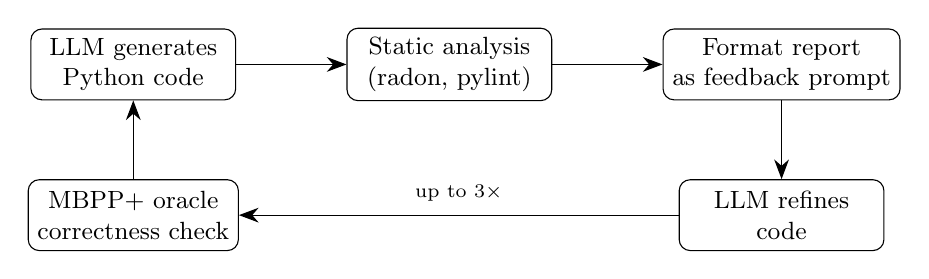
\begin{tikzpicture}[
      node distance=10mm and 14mm,
      box/.style={rectangle,draw,rounded corners,align=center,
                  minimum height=9mm,minimum width=26mm,font=\small},
      arr/.style={-{Stealth[length=2.5mm]}}]
    \node[box] (gen)   {LLM generates\\Python code};
    \node[box,right=of gen] (analyze) {Static analysis\\(radon, pylint)};
    \node[box,right=of analyze] (feedback) {Format report\\as feedback prompt};
    \node[box,below=of feedback] (refine) {LLM refines\\code};
    \node[box,below=of gen] (test) {MBPP+ oracle\\correctness check};
    \draw[arr] (gen) -- (analyze);
    \draw[arr] (analyze) -- (feedback);
    \draw[arr] (feedback) -- (refine);
    \draw[arr] (refine) -- node[midway,above=0.5mm,font=\scriptsize]{up to 3$\times$} (test);
    \draw[arr] (test) -- (gen);
  \end{tikzpicture}
  \caption{Iterative static-analysis feedback pipeline.}
  \label{fig:pipeline}
\end{figure*}

\subsection{Task Set and Correctness Oracle}
\label{sec:taskset}
Tasks are drawn from the sanitized MBPP problems~\citep{austin2021mbpp} and are
evaluated with MBPP+. EvalPlus~\citep{liu2023evalplus} is a framework that augments
a benchmark with a substantially larger, automatically generated set of test
inputs; the paper applies it to HumanEval and names MBPP as future work. MBPP+ is
the result of that later application and is distributed with the EvalPlus tool,
version~0.3.1~\citep{evalplus_tool}, which is the version used here. The augmented
suite makes the correctness check considerably more rigorous than the handful of
tests shipped with the original problems, and the size of that difference was
measured directly on the task set used here: across the 63 tasks the benchmark's
own inputs number 193, against 6519 added by the augmentation. To ensure every task offers
structural headroom for the feedback loop to act on, tasks are filtered by an
objective, reproducible criterion applied to their reference solution: cyclomatic
complexity $\geq 3$ and $\geq 5$ lines of code, excluding tasks that require file
or network input/output. The filter is applied to the full pool of 378 tasks
distributed with the tool, is deterministic, and involves no sampling or manual
selection step: it yields exactly \textbf{63 tasks}. Because the criterion is
evaluated on the reference solutions, which are fixed properties of the benchmark,
the task set was settled before any code was generated and never revised
afterwards. These are stratified by the same
reference-solution complexity into a \emph{lower} group (cyclomatic complexity
3--4, $n=40$) and a \emph{higher} group (cyclomatic complexity $\geq 5$, $n=23$) so
that the effect of the loop can be analyzed by difficulty. The strata are therefore
a property of the benchmark tasks, fixed before any code was generated, and not of
the model's own baseline output. Correctness is decided by an
EvalPlus-style oracle: a solution passes only if, for every base and extended
input, its output matches the canonical reference solution (with floating-point
tolerance) and it raises no exception. The identical oracle is applied at every
iteration, which is how the study checks that code still works after
refinement: H3 is evaluated by comparing each task's baseline and final pass/fail
outcome under exactly the same inputs, and the McNemar
test~\citep{mcnemar1947} then operates on the
resulting discordant pairs (\cref{sec:results}). Each candidate is executed in an
isolated subprocess that is killed as a process group on timeout, with a second
in-process alarm inside the harness, so a non-terminating solution is recorded as a
failure rather than stalling the run.

Because H3 rests entirely on this oracle, the oracle itself was checked rather than
assumed. Submitting each task's own reference solution to it as though it were a
candidate, all 63 pass; submitting a deliberately corrupted variant of each
reference, all 63 fail. The augmented inputs also demonstrably discriminate: 40 of
the 63 baseline solutions satisfy the benchmark's original inputs, but 12 of those
are then caught by the augmentation, which is what reduces the baseline pass count
to the 28 reported in \cref{sec:results}. Almost a fifth of the task set would
therefore have been scored correct under the unaugmented benchmark.

\subsection{Loop Configurations}
\label{sec:configs}
Three configurations of the feedback loop are compared against the shared
baseline, all using the identical model, sampling parameters, task set, and
iteration cap. They differ only in the feedback prompt and in the policy that
decides which version is carried into the next iteration:
\begin{itemize}
  \item \textbf{Unguarded (comment-stripping).} The refactor prompt does not
    instruct the model to preserve existing comments. The label describes the
    observed outcome rather than the instruction: across the archived run the
    comment and docstring lines in the generated solutions fall from 268 at the
    baseline to 78 at the final iteration, against a rise to 324 under the
    comment-preserving prompt. Contrasting the two configurations tests whether
    comment handling affects the Maintainability Index.
  \item \textbf{Unguarded (comment-preserving).} Identical to the above except for
    one appended sentence instructing the model to keep any existing docstring and
    comments. Every other element of the prompt, including the requirement to preserve the
    exact function signature and behavior, is shared with the
    comment-stripping configuration, which is what makes the pair a controlled
    contrast. In both unguarded configurations the latest refactor is always
    carried forward, even if it fails the correctness check.
  \item \textbf{Correctness-guarded.} This configuration uses the
    comment-preserving prompt, so it differs from the second configuration in its
    carry-forward policy alone. The correctness check acts as a gate,
    mirroring a continuous-integration quality gate; the same principle as the
    fitness gate of Blyth et al.~\citep{blyth2025scam}, applied here to
    structural-metric refactoring rather than to linter
    violations. A refactor is accepted only
    if it still passes the oracle; otherwise it is rejected and the loop rolls
    back to the last accepted (still-correct) version, and the model is informed
    on the next attempt that its change altered behavior. That notice is not
    merely informative but structurally necessary: because decoding is greedy and
    the seed is fixed, rolling back and re-prompting with a byte-identical prompt
    would regenerate the same rejected refactor indefinitely. Adding the notice
    perturbs the prompt, which is what allows a retry to differ from the attempt it
    replaces. (The one exception is a
    task the baseline never solved: while the carried-forward version is still
    failing, any candidate is accepted, since correctness cannot regress below an already-failing baseline; this lets the loop repair such a task if it
    can.)
    By construction, final correctness can therefore never fall below the baseline.
\end{itemize}

A further comparison isolates the \emph{content} of the feedback rather than the
carry-forward policy. In all three configurations above, the model is shown its own
previous code together with the static-analysis findings. A \emph{code-blind}
variant instead withholds the previous code and supplies only the scalar findings
of the previous attempt---the Maintainability Index, the cyclomatic and cognitive
complexity totals, and the Pylint issue counts by category---asking the model to
generate a fresh, simpler solution to the same task. This tests whether the
improvement is driven by the model editing its own code or merely by being told
that its previous attempt was too complex. The code-blind variant is run in both an
unguarded and a correctness-guarded form and is reported as a secondary ablation
(\cref{sec:blind}).

\subsection{Frozen Protocol}
All generation parameters are fixed in a single version-controlled configuration
file and applied unchanged to every run: model \texttt{qwen2.5-coder:7b}
(Q4\_K\_M quantization), temperature~0, seed~42, a context window of 4096 tokens,
and an iteration cap of three. Because the model is served locally with greedy
decoding and a fixed seed, generations are not subject to provider drift, and the
generated code and per-iteration metrics are retained for every task and
iteration so that each reported value can be traced to the artifact that produced
it.

One limit on exact replication should be stated plainly: an Ollama tag identifies a
model by name rather than by content, so a future pull of \texttt{qwen2.5-coder:7b}
is not guaranteed to resolve to the same weights. The weights actually used are
nonetheless pinned by digest. The identifier \texttt{ollama list} reports for the
tag is \texttt{dae161e27b0e}, and the model layer it references is
\texttt{sha256:60e05f21\ldots} at 4.68\,GB; both are recorded in the configuration
file alongside the sampling parameters. These digests were read back from the local
model store after the experiment rather than logged during it, so the supporting
evidence that one set of weights served every run is that the manifest and the
weight blob both carry an unmodified timestamp preceding the earliest run; the tag
was pulled once and never re-pulled. A replication can therefore check that it
loaded the same weights by comparing these digests against its own, which the tag
alone would not allow.

\subsection{Artifacts and What Is Reproducible}
\label{sec:artifacts}
Two different claims are often both called reproducibility, and only the first of
them is exact here.

\emph{Recomputation from the archived artifacts is exact.} Every solution the model
produced is retained---1260 files across the five configurations, one per task and
iteration---together with the metric values recorded for it at run time. Every
number reported in this thesis is derived from those files by a deterministic
analysis script, and re-measuring all 1260 archived solutions reproduces all of the
recorded metric values exactly. A reader can therefore trace any reported figure to
the specific solution that produced it, and can confirm the statistics offline
without a model, a network connection, or an API key.

\emph{Re-running generation is approximate.} Single-shot generation is
deterministic: under greedy decoding with a fixed seed, the baseline iteration is
byte-identical across all five configurations. A multi-step trajectory is not
equally stable, because once any intermediate iteration differs the later ones can
diverge from it. A fresh run of the loop should therefore be expected to reproduce
the direction and rough magnitude of the effects reported here rather than the exact
values, and the figures quoted throughout are properly read as measurements of the
archived runs rather than as constants of the method. The consequences of this for
the study's conclusions are taken up in \cref{sec:limitations}.

% !TeX root = ../paper.tex

\section{Evaluation and Discussion}
\label{sec:results}

Results are organized by hypothesis. All figures report the per-task paired change
between the no-feedback baseline and the final iteration, across the three loop
configurations of \cref{sec:configs}. Two significance tests are used: the
Wilcoxon signed-rank test~\citep{wilcoxon1945signedrank} for the paired metric
changes (H1, H2), and an exact (binomial) variant of the McNemar
test~\citep{mcnemar1947} for the change in
functional correctness (H3). Both are non-parametric
and paired, which suits the bounded, non-normal metrics and the small sample.
Because a family of twelve tests is reported---the three primary metrics and the
correctness test, each across the three configurations---every $p$-value is
additionally assessed against a Bonferroni-corrected
threshold~\citep{dunn1961multiple} of
$\alpha^\ast = 0.05/12 = 0.00417$ to control the family-wise error rate. A
summary is given in \cref{tab:results}, where the $p$-values that remain
significant after this correction are marked with a dagger ($\dagger$).

Every value below measures the archived runs (\cref{sec:artifacts}) and recomputes
from the retained solutions exactly; a fresh run reproduces the direction and
approximate size of these effects but not their precise figures, so the discussion
rests on the sign, significance, and ordering of the effects rather than their exact
magnitudes.

\subsection{Baseline Results}
The baseline model solves \textbf{28 of 63 tasks} (44\,\%) under the MBPP+ oracle.
Its generated code already scores well: the median baseline Maintainability Index
is 95.4, and 46 of 63 solutions reach at least 90, though \cref{sec:results}
shows how much of that is comment credit.

\begin{table*}[t]
  \centering
  \caption{Effect of three feedback-loop configurations on 63 tasks. Metric
    columns report the median per-task change (final $-$ baseline) and the
    two-sided Wilcoxon $p$; correctness reports the baseline$\rightarrow$final
    pass count and the exact McNemar-type $p$. For MI, higher is better (a negative
    change is a decline); for CC and CogC, lower is better (a negative change is
    an improvement). A dagger ($\dagger$) marks $p$-values below the
    Bonferroni-corrected threshold $\alpha^\ast = 0.05/12 = 0.00417$.}
  \label{tab:results}
  \begin{tabular}{lccccc}
    \toprule
    & \textbf{Correctness} & \multicolumn{2}{c}{\textbf{MI (H1)}}
      & \textbf{CC (H2)} & \textbf{CogC (H2)} \\
    \cmidrule(lr){3-4}
    \textbf{Configuration} & base$\rightarrow$final ($p$) & med.\ $\Delta$ & $p$
      & med.\ $\Delta$ ($p$) & med.\ $\Delta$ ($p$) \\
    \midrule
    Unguarded, comment-stripping    & $28\!\to\!23$ ($.13$)  & $-3.0$ & $<.001^\dagger$ & $0$ ($.0036^\dagger$) & $-1$ ($<.001^\dagger$) \\
    Unguarded, comment-preserving   & $28\!\to\!22$ ($.07$)  & $-3.4$  & $<.001^\dagger$ & $0$ ($.02$)    & $0$ ($<.001^\dagger$) \\
    Correctness-guarded             & $28\!\to\!\mathbf{29}$ ($1.0$) & $-1.1$ & $<.001^\dagger$ & $0$ ($.03$)  & $0$ ($<.001^\dagger$) \\
    \bottomrule
  \end{tabular}
\end{table*}

\subsection{Effect on Maintainability (H1)}
The Maintainability Index does not improve under any configuration; it declines
significantly in all three (\cref{fig:deltas}, left). The
decline is, tellingly, essentially the same whether the refactor prompt
strips comments or preserves them: a median of $-3.0$ points in the
comment-stripping configuration versus $-3.4$ in the comment-preserving one. A
direct per-task comparison of the two confirms this; their final Maintainability
Indices do not differ significantly (Wilcoxon $p=.13$). That similarity is not,
however, evidence that comments are irrelevant. Comment density is high at the
baseline (mean 49\,\%) and moves sharply both ways, to 19\,\% under the stripping
prompt and to 85\,\% under the preserving one, while the Index's comment term is
non-monotonic and peaks near 58\,\%~\citep{coleman1994maintainability,radon_docs}.
A baseline sitting at that maximum therefore loses points in \emph{either}
direction: the term falls by a mean of 14.2 points under stripping and 8.8 under
preserving, and at the median baseline ratio it contributes about 29 points on its
own, so the ceiling is largely its artifact too. Comment handling is thus the dominant driver of every MI figure
reported here; with the term held fixed, the mean structural component instead rises
slightly in all three configurations. Combined with the validity limitations
documented by Heitlager et al.~\citep{heitlager2007maintainability}, the decline is
best read as evidence that the MI is an unsuitable outcome metric here, not that
the loop harms maintainability. The Index is therefore reported for completeness
but treated as secondary; cognitive complexity is the primary maintainability
signal in what follows.

\subsection{Effect on Complexity (H2)}
Cognitive complexity improves. Although its median change is zero or $-1$---most of
the 63 tasks are simple enough that little or no reduction is possible---the change
is highly significant in every configuration ($p<.001$; \cref{fig:deltas}, right),
because among the tasks that do change, reductions dominate overwhelmingly. In the
correctness-guarded configuration, 26 tasks reduce their cognitive complexity and
only one increases it. Of the 63 tasks, 36 show no change at all; the Wilcoxon
test discards these zero-difference pairs as uninformative and evaluates only the
27 tasks that did change. Among those 27, a 26:1 split in favor of reductions is
highly unlikely to arise by chance, which is what drives the significance despite
the zero median. The effect is strongest where there is structural headroom:
in the higher-complexity stratum of the guarded loop the median change is $-1$ and
remains significant ($p=.002$), though this stratum analysis is exploratory and is
not part of the corrected family. Individual cases are substantial; for example one task falls from a
cognitive complexity of 15 to 2 while remaining correct. \Cref{fig:cogcscatter}
shows this task-by-task: most points lie on or below the diagonal, and the largest
reductions occur at the highest baseline values.

Cyclomatic complexity behaves similarly but more weakly. Its reductions are
smaller: at the uncorrected level they are significant in all three configurations
(comment-stripping $p=.0036$, comment-preserving $p=.02$, guarded $p=.03$), but
after Bonferroni correction only the comment-stripping configuration remains
significant. This divergence between the two complexity
metrics is expected: the feedback
prompt targets nested and redundant control flow, which cognitive complexity
penalizes more directly than cyclomatic complexity.

\begin{figure*}[t]
  \centering
  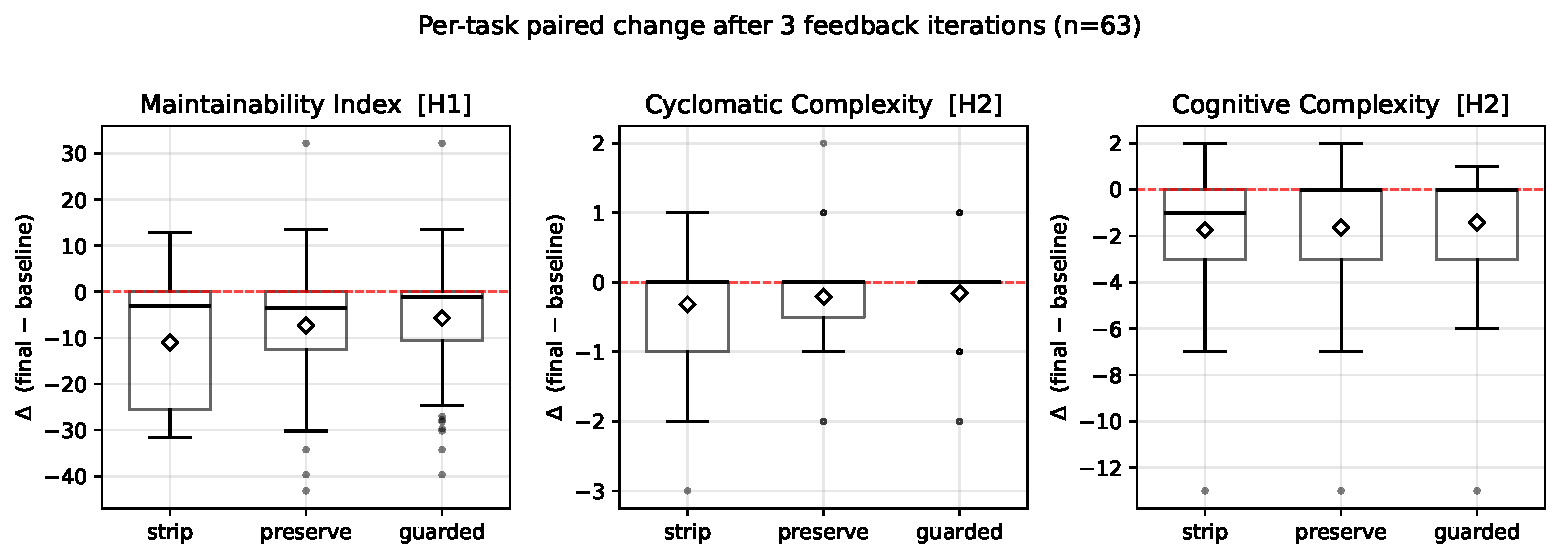
\includegraphics[width=\textwidth]{figures/fig_delta_boxplots}
  \caption{Per-task paired change (final $-$ baseline) for each metric and
    configuration. The dashed line marks no change; diamonds mark means. The
    Maintainability Index (left) declines modestly and by a similar amount in
    every configuration; cyclomatic complexity (middle) barely moves; cognitive
    complexity (right) concentrates below zero, indicating reductions.}
  \label{fig:deltas}
\end{figure*}

\subsection{Qualitative Example: De-nesting Reduces Cognitive Complexity}
\label{sec:example}
\Cref{fig:example} makes the aggregate cognitive-complexity result concrete on a
single task (Mbpp/245, the maximum sum of a bitonic subsequence). The baseline
solution (a) computes two auxiliary arrays with doubly nested loops whose inner
bodies guard an accumulator update with a compound \texttt{if}; this deep nesting
is what cognitive complexity penalizes, and the solution scores 15. Under the
correctness-guarded loop the model replaced each inner loop with a generator
expression inside \texttt{max(\dots, default=\dots)}, removing the nesting while
computing the same values; cognitive complexity falls to 2 and the solution still
passes the MBPP+ oracle. This single example also illustrates why the two
complexity metrics diverge (\cref{sec:supp}): \emph{cyclomatic} complexity is unchanged at 10; the number of
independent branches is essentially the same, yet \emph{cognitive} complexity drops by 13, because it is the nesting, not the branch
count, that the refactor removed. The Maintainability Index rises from 78.5 to
92.0 and the code shortens from 18 to 9 lines, but the readability gain that
cognitive complexity captures is the substantive change.

\begin{figure*}[t]
  \centering
  \begin{minipage}{\textwidth}
  \footnotesize (a) Baseline solution --- cognitive complexity 15, cyclomatic 10, MI 78.5.
  \begin{lstlisting}[basicstyle=\ttfamily\footnotesize,numbers=none]
def max_sum(arr):
    n = len(arr)
    inc = [0] * n
    dec = [0] * n
    for i in range(n):
        inc[i] = arr[i]
        for j in range(i):
            if arr[i] > arr[j] and inc[i] < inc[j] + arr[i]:
                inc[i] = inc[j] + arr[i]
    for i in range(n-1, -1, -1):
        dec[i] = arr[i]
        for j in range(i+1, n):
            if arr[i] > arr[j] and dec[i] < dec[j] + arr[i]:
                dec[i] = dec[j] + arr[i]
    max_sum_bitonic = 0
    for i in range(n):
        max_sum_bitonic = max(max_sum_bitonic, inc[i] + dec[i] - arr[i])
    return max_sum_bitonic
  \end{lstlisting}
  \vspace{0.4em}
  \footnotesize (b) After correctness-guarded feedback --- cognitive complexity 2, cyclomatic 10, MI 92.0.
  % scriptsize, not footnotesize: the two generator-expression lines are ~97 chars
  % and wrapped mid-subscript at footnotesize, which read as broken Python. The code
  % is the model's output and is shown verbatim, so it is the type size that gives.
  \begin{lstlisting}[basicstyle=\ttfamily\scriptsize,numbers=none]
def max_sum(arr):
    n = len(arr)
    inc = [arr[i] for i in range(n)]
    dec = [arr[i] for i in range(n)]
    for i in range(1, n):
        inc[i] = max((inc[j] + arr[i] for j in range(i) if arr[i] > arr[j]), default=arr[i])
    for i in range(n-2, -1, -1):
        dec[i] = max((dec[j] + arr[i] for j in range(i+1, n) if arr[i] > arr[j]), default=arr[i])
    return max(inc[i] + dec[i] - arr[i] for i in range(n))
  \end{lstlisting}
  \end{minipage}
  \caption{A representative correctness-preserving refactor from the guarded loop
    (comments omitted for space). Replacing the nested inner loops with generator
    expressions removes the deep nesting: cognitive complexity falls from 15 to 2
    while cyclomatic complexity is unchanged at 10, and all MBPP+ tests still pass.}
  \label{fig:example}
\end{figure*}

\subsection{Effect on Functional Correctness (H3)}
The unguarded configurations trend toward losing correct solutions, from 28 down
to 23 and 22, but neither change is statistically significant (McNemar
$p=.13$ and $p=.07$). This is an important limit on the claim: at this sample size,
the data do not establish that the unguarded loop significantly harms correctness,
only that it does not improve it and shows a downward trend. The counts are
nonetheless worth reading in proportion rather than in the aggregate: of the 28
solutions that were correct at the baseline, 6 and 7 respectively were broken by refactoring, between a fifth and a quarter of everything the model had already got
right. Whether or not that reaches significance on 63 tasks, it is the practical
risk the gate is designed to remove. The
correctness-guarded configuration ends at 29 correct solutions with zero
regressions. This is a design guarantee rather than a
statistical result: the gate rejected 13 of 189 refactors that broke behavior---12
of them in the lower-complexity stratum, where the model tends to over-refactor
simple functions---and rolled each one back to its last correct version.

The gate also works in the other direction, which is why the guarded run ends
\emph{above} its baseline. On one task (Mbpp/167, ``next power of 2'') the baseline
solution initialized its accumulator to $0$ and then doubled it with a left shift,
so the loop condition never advanced and the oracle recorded a timeout as a
failure. A later refactor initialized the accumulator to $1$ instead, which is
correct; the gate verified the fix against the oracle and locked it in. The gate is
therefore a ratchet on correctness rather than merely a brake: it can hold or
improve the pass count but, by construction, never reduce it.

\begin{figure}[t]
  \centering
  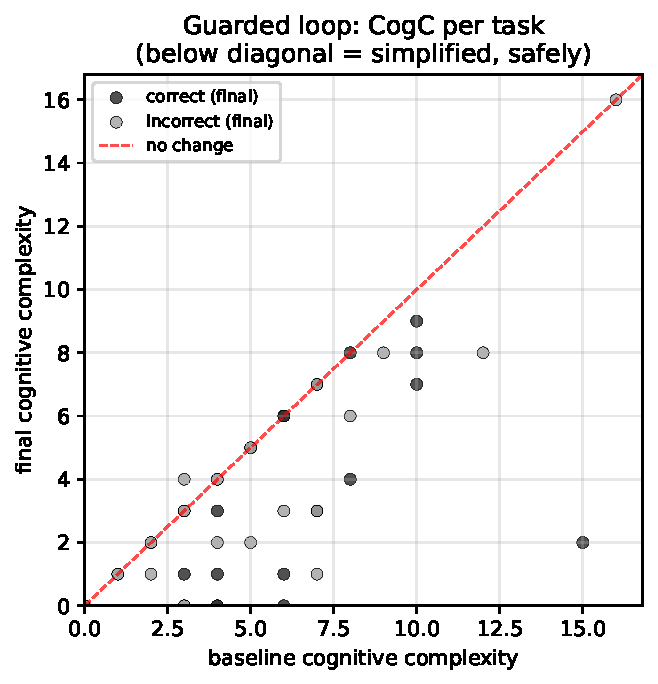
\includegraphics[width=0.72\columnwidth]{figures/fig_cogc_scatter}
  \caption{Guarded loop: baseline versus final cognitive complexity for all 63
    tasks. Points below the diagonal are simplified. No task that passes the
    baseline oracle fails at the final iteration; tasks failing both are included.}
  \label{fig:cogcscatter}
\end{figure}

\subsection{Iteration Dynamics}
\label{sec:trajectory}
\Cref{fig:trajectory} tracks how the metrics evolve across the three feedback
iterations. The effect is concentrated almost entirely in the first iteration:
mean cognitive complexity and the Maintainability Index both move at iteration~1
and then change little through iterations~2 and~3, in every configuration. This
holds at the task level too---among the tasks whose cognitive complexity changes at
all, most reach their final value already after one iteration (27 of 39 for
comment-stripping, 24 of 32 for comment-preserving, and 20 of 27 for the guarded
loop), with only a handful first improving at the second or third iteration. The
loop therefore behaves close to a single-shot refactor. The three-iteration budget
is consequently not a binding constraint for most tasks; it mainly provides
headroom for the minority that improve later and, in the guarded loop, for retries
after a rejected refactor. A smaller cap would capture most of the observed
benefit, and a substantially larger one would be unlikely to add much, which is the empirical justification for the fixed cap of three.

\begin{figure}[t]
  \centering
  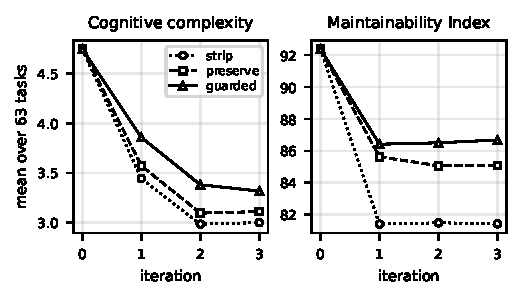
\includegraphics[width=\columnwidth]{figures/fig_trajectory}
  \caption{Mean cognitive complexity (left) and Maintainability Index (right) at
    each iteration (0~=~baseline), one line per configuration. Both change chiefly
    at the first iteration and then plateau, in all three configurations.}
  \label{fig:trajectory}
\end{figure}

\subsection{Supplementary Metrics}
\label{sec:supp}
Beyond the three primary metrics, the pipeline records lines of code (LOC),
Halstead volume and effort, and Pylint issue counts at no additional measurement
cost. These are reported here as descriptive corroboration; they are not part of
the hypothesis family and carry no significance test. Because all three
configurations share the identical baseline generation, their baseline medians
coincide (\cref{tab:supp}).

Two of these measures independently reinforce the interpretation of the primary
results. First, source lines of code barely move and do so uniformly; the median falls from 9 to 7 in every configuration, including comment-stripping. Because SLOC excludes comments and multiline strings, that uniformity says nothing
about comment volume; the component analysis above shows the comment ratio is what
drives the MI decline. Second, Halstead
volume and effort are effectively flat (median change $\approx 0$) in every
configuration: the loop restructures control flow without materially changing
program size or vocabulary. This is exactly the signature expected when cognitive
complexity, which penalizes nesting and control structure, falls while size-based
measures do not, and it argues against the complexity reduction being an artifact
of the code simply getting smaller. Pylint issue counts decline modestly (median 6
to 4--5). This last figure carries the least evidential weight of any reported
here, because Pylint is the loop's own feedback source: the model is told which
findings it triggered, so a subsequent fall in those counts partly restates the
instruction rather than measuring an independent improvement. It is noted as a
side effect and nothing in the argument depends on it.

\begin{table}[t]
  \centering
  \footnotesize
  \setlength{\tabcolsep}{4pt}
  \caption{Supplementary metrics (descriptive; not in the hypothesis family),
    reported as median baseline$\rightarrow$median final per configuration
    (comment-stripping / comment-preserving / correctness-guarded). Baselines
    coincide because the three configurations share one baseline generation. LOC
    is source lines of code (\texttt{radon raw} SLOC); Pylint issues is the total
    of convention, refactor, warning, and error messages.}
  \label{tab:supp}
  \begin{tabular}{lccc}
    \toprule
    & \textbf{Strip} & \textbf{Preserve} & \textbf{Guarded} \\
    \midrule
    LOC (SLOC)      & $9\!\to\!7$         & $9\!\to\!7$         & $9\!\to\!7$ \\
    Halstead vol.   & $62.3\!\to\!57.1$   & $62.3\!\to\!64.7$   & $62.3\!\to\!64.7$ \\
    Halstead eff.   & $140.1\!\to\!142.4$ & $140.1\!\to\!142.4$ & $140.1\!\to\!142.4$ \\
    Pylint issues   & $6\!\to\!4$         & $6\!\to\!4$         & $6\!\to\!5$ \\
    \bottomrule
  \end{tabular}
\end{table}

\subsection{Synthesis}
Taken together, the three configurations answer the research question with a
qualified yes. The feedback loop produces a statistically significant reduction in
cognitive complexity, one that survives Bonferroni correction for multiple
comparisons in every configuration, without a statistically significant loss of
functional correctness, and the correctness-guarded variant turns the absence of
regression into a guarantee. It does not improve the Maintainability Index, but that decline tracks the Index's
comment term rather than structural quality, which, with its documented validity
limitations~\citep{heitlager2007maintainability}, makes it a sign of the metric's
unsuitability here rather than a failing of the method. The practical cost of the guarantee is small: the
guarded loop forgoes a few complexity reductions that were only achievable by
altering behavior (12 tasks reduced cyclomatic complexity, against 16 under the
comment-preserving unguarded loop that shares its prompt), in exchange for
eliminating every correctness regression. A follow-up
ablation (\cref{sec:blind}) shows that this complexity reduction does not even
require showing the model its own code.

\subsection{Feedback Content: Is the Generated Code Needed?}
\label{sec:blind}
The configurations above all feed the model its previous code together with the
static-analysis findings. To test whether the code is what drives the effect, a
\emph{code-blind} variant withholds the previous code and supplies only the
scalar findings of the previous attempt, asking for a fresh, simpler solution
(\cref{sec:configs}). Because this variant addresses a distinct, secondary
research question rather than the pre-specified primary hypotheses, its tests are
treated as a separate multiplicity family with their own correction. It is
compared against the
code-aware comment-preserving loop, though the two prompts also differ in comment
handling, so this ablates the feedback package rather than code visibility alone.

The central result is that the code is \emph{not} needed for the complexity
reduction. The code-blind loop reduces cognitive complexity significantly (median
$-1$, $p<.001$), and a per-task comparison of the two final versions shows no
significant difference from the code-aware loop ($p=.65$); the Maintainability
Index declines almost identically in both ($-3.4$ points). Withholding the code
does, however, make the unguarded loop noisier on correctness: because it
re-derives each solution from scratch rather than editing a known-correct one, it
regresses eight tasks and repairs three, against the code-aware loop's seven and
one (\cref{tab:blind}). The code-blind loop ends at 23 correct solutions and the code-aware at 22, neither change is statistically
significant, but the code-blind
loop clearly takes larger correctness risks in both directions.

This is precisely the risk the correctness gate is designed to absorb, and it
does. The guarded code-blind loop rejects every behavior-breaking regeneration, so
it records \emph{zero} regressions; and because blind regeneration is a coarser
operation that occasionally rewrites a broken baseline into a correct solution, it
even repairs three tasks, ending at 31 correct, slightly above the guarded
code-aware loop's 29. Its cognitive-complexity reduction is preserved ($p=.005$)
and again statistically indistinguishable from the code-aware loop ($p=.43$). The
practical conclusion is that showing the model its own code is unnecessary for the
complexity benefit, and that a lightweight correctness gate makes code-blind
regeneration not merely safe but, on this sample, marginally better for
correctness.

\begin{table}[t]
  \centering
  \footnotesize
  \setlength{\tabcolsep}{2pt}
  \caption{Code-blind ablation (secondary family, $n=63$), compared with the
    code-aware comment-preserving loop. Correctness reports
    baseline$\rightarrow$final with the exact McNemar-type $p$; CogC and MI report the
    median per-task change and the Wilcoxon $p$. A dagger ($\dagger$) marks
    $p$-values below this family's Bonferroni threshold
    $\alpha^\ast = 0.05/8 = 0.00625$.}
  \label{tab:blind}
  \begin{tabular}{lccc}
    \toprule
    \textbf{Configuration} & \textbf{Correct.} & \textbf{CogC} & \textbf{MI} \\
    & base$\rightarrow$final & med.\ $\Delta$ ($p$) & med.\ $\Delta$ ($p$) \\
    \midrule
    Code-aware, ungu.  & $28\!\to\!22$ & $0$ ($<.001^\dagger$) & $-3.4$ ($<.001^\dagger$) \\
    Code-blind, ungu.  & $28\!\to\!23$ & $-1$ ($<.001^\dagger$) & $-3.4$ ($.002^\dagger$) \\
    Code-aware, guard. & $28\!\to\!29$ & $0$ ($<.001^\dagger$) & $-1.1$ ($<.001^\dagger$) \\
    Code-blind, guard. & $28\!\to\!\mathbf{31}$ & $0$ ($.005^\dagger$) & $-1.4$ ($.008$) \\
    \bottomrule
  \end{tabular}
\end{table}

% !TeX root = ../paper.tex

\section{Limitations and Future Work}
\label{sec:limitations}

The findings hold under a specific set of choices. This section states the most
consequential of those bounds, grouped by the kind of validity each threatens. Two of these, the unsuitability of the Maintainability
Index and the limited power of the correctness test, are load-bearing enough that the conclusions are already phrased
around them.

\subsection{Construct Validity: Does the Measurement Capture Maintainability?}

\paragraph{The Maintainability Index.} Beyond the validity critique already
discussed~\citep{heitlager2007maintainability}, the Index proved in this study
uninformative rather than misleading: it moved almost identically across
configurations, whether or not comments were stripped, because its comment term
dominates the score at this code size, so it did not usefully discriminate between
the loop's outputs. A comment-normalized or volume-controlled measure would be a more
informative outcome metric.

\paragraph{Tool-specific operationalization.} Each metric is defined here by the
tool that computed it: the Index is \texttt{radon}'s normalized 0--100 derivative
rather than Coleman et al.'s unbounded
polynomial~\citep{coleman1994maintainability,radon_docs}, and cognitive complexity
is \texttt{complexipy}'s implementation of Campbell's
specification~\citep{cognitivecomplexity,complexipy_tool}. Both tools are pinned to the
versions used, so that a replication measures with the same implementation. The
results are therefore statements about these operationalizations rather than about
the constructs in the abstract.

\paragraph{Metric-level, not human, maintainability.} Maintainability is assessed
only through static metrics; perceived readability and human effort were not
measured. The Pylint counts are weaker still, being the loop's own feedback source
(\cref{sec:supp}), and no claim here rests on them; the model is shown its complexity
totals but is never given the Maintainability Index as a target, and the
cognitive-complexity result is a measured consequence of the refactoring instruction
rather than a restatement of it.

\subsection{Internal Validity: Could the Effect Have Another Cause?}

\paragraph{Code size as an alternative explanation.} The obvious rival explanation
is that the code simply became shorter; the supplementary measures argue against
it (\cref{sec:supp}), as the loop restructures control flow rather than shrinking
programs.

\paragraph{A single feedback prompt.} The prompt wording was not varied
systematically: the only variation tested was comment handling, whose effect on the
Index was not significant ($p=.13$). The study therefore provides no evidence about
sensitivity to the rest of the phrasing---which findings are shown, in what order,
and how forcefully.

\paragraph{Two factors inside the correctness gate.} The guarded configuration
changes two things at once: it rolls back a failing refactor, and it tells the model
its change altered behavior. The zero-regression guarantee follows from the rollback
alone, but the gate's effect on the complexity results cannot be attributed to
either factor separately; separating them would need a third condition that rolls
back silently.

\paragraph{Limits of the correctness oracle.} MBPP+ inputs are generated
automatically, so passing the oracle establishes agreement with the reference
solution on the tested inputs rather than correctness in general; a refactor that
breaks behavior only on an untested input would be recorded as correct. The oracle
also treats a timeout as a failure, which is the desired behavior for a
non-terminating refactor but means a genuinely slow solution could be scored the
same way. Neither limitation is specific to this study---it is inherited from the
benchmark---but both bound how strong ``still correct'' is as a claim.

\paragraph{The iteration cap.} The cap of three was fixed in advance as a budget,
not derived from a power analysis. The trajectory analysis
(\cref{sec:trajectory}) later showed it was not binding for most tasks, but that is
a post-hoc justification and does not establish that a larger budget would change
nothing.

\subsection{External Validity: How Far Does This Generalize?}

\paragraph{Scope of the sample.} The study uses a single model
(Qwen2.5-Coder-7B-Instruct) at a single fixed seed, on 63 short benchmark tasks
(23 in the higher-complexity stratum). Short, self-contained tasks have limited
explanatory power for large software systems, so all claims are scoped strictly to
this experimental setting. Whether the cognitive-complexity effect generalizes to
other model families and sizes was not tested and is left to future work.

\paragraph{One decoding configuration and one quantization.} Generation used greedy
decoding at temperature~0 and the Q4\_K\_M quantization throughout. Both were chosen
for reproducibility, and both plausibly matter: quantization may affect output
quality, and sampling at a higher temperature would introduce the run-to-run
variation that temperature~0 deliberately removes. Neither was varied, so the
results describe one point in that space.

\paragraph{Model identity.} An Ollama tag names a model rather than fixing its
content. The digests of the weights used are recorded (\cref{sec:method}) so a
replication can check them, but they were read back after the fact, and the evidence
that one set of weights served all five runs is timestamp-based.

\subsection{Statistical Conclusion Validity}

\paragraph{Power and multiplicity.} A family of twelve tests is
reported (the three primary metrics and the correctness test, each across the
three configurations). To control the family-wise error rate, a Bonferroni
correction is applied, giving an adjusted threshold of
$\alpha^\ast = 0.05/12 = 0.00417$. The cognitive-complexity reductions and the
Maintainability-Index movements remain significant under this correction in every
configuration; only the weaker cyclomatic-complexity results in the guarded and
comment-preserving loops fall away. Bonferroni controls the family-wise error rate
at $\alpha = 0.05$ regardless of the dependence among the tests. Several outcomes
here are computed from the same tasks and the configurations share a common
baseline, so the tests are not independent; the correction may consequently be
conservative, although the degree of that conservatism is not quantified here. A
step-down (Holm) correction~\citep{holm1979} rejects the
same set. The
code-blind ablation (\cref{sec:blind}) is kept in a separate secondary family of
eight tests with its own threshold ($\alpha^\ast = 0.05/8 = 0.00625$), under
which both code-blind cognitive-complexity reductions survive; were the two
families instead pooled into a single set of twenty tests
($\alpha^\ast = 0.05/20 = 0.0025$), the guarded code-blind result ($p=.005$) and the
comment-stripping cyclomatic-complexity result ($p=.0036$) would both cease to be significant; the unguarded code-blind result ($p<.001$)
would still clear it, and the cognitive-complexity and Maintainability-Index
conclusions for the three primary configurations are unchanged. The per-stratum
analyses are treated as secondary and exploratory. Independently, with 63 tasks
and only a handful of discordant pairs the correctness (McNemar) test has low
power, so the non-significant downward trend of the unguarded loop should not be
over-interpreted.

\subsection{Reproducibility and Artifact Availability}
\label{sec:repro}

\paragraph{What is reproducible, and how exactly.} As set out in
\cref{sec:artifacts}, recomputation and re-running are different claims. All 1260
retained solutions re-measure to their recorded values, so each figure traces to a
specific artifact and the statistics can be re-derived offline. Re-running
generation is weaker: the baseline is byte-identical across configurations, but a
multi-step trajectory can diverge once any intermediate iteration differs. The
quantities above are therefore measurements of a single archived run per
configuration, not constants a fresh execution will reproduce digit for digit.

\paragraph{An incident that shaped this position.} The distinction just drawn was
learned rather than adopted on principle. Two loop runners originally wrote their
generated code to the same filename pattern, so the second silently overwrote the
first run's saved solutions; the overwrite was found by an integrity audit before
submission and the affected configurations were re-run under collision-free names.
On the fresh runs a substantially larger Maintainability-Index effect previously
recorded for the comment-stripping configuration did not reproduce; it fell from roughly $-16$ points to the $-3.0$ reported here, and the strip-versus-preserve
difference became non-significant. That figure and the ablation argument built on it
were withdrawn, and the fresh runs adopted as canonical. The instability was
specific to multi-step trajectories, which is why this thesis rests its conclusions
on effect direction and significance rather than on precise magnitudes.

\subsection{Future Work}

The bounds above suggest the following directions, roughly in order of how directly
they address a limitation identified here.

\begin{itemize}
  \item \textbf{Replicate across models.} Repeat the study on structurally messier
    code generators to test whether the cognitive-complexity effect is a property of
    the technique or of this model.
  \item \textbf{Vary the prompt and pre-register.} Measure sensitivity to which
    findings are shown and how the instruction is phrased---the factor held fixed
    here---and fix the metric family, correction scheme, and iteration budget in
    advance.
  \item \textbf{Adopt a volume-controlled maintainability measure.} A metric that
    does not conflate code size and comment density with structural quality would
    give H1 an informative outcome variable instead of one at its ceiling.
  \item \textbf{Add human raters.} Test whether the measured reductions correspond
    to code developers find easier to read and change, and decompose the gate with a
    silent-rollback condition.
  \item \textbf{Scale beyond self-contained functions.} Apply the loop to
    repository-level code, where maintainability matters most and the
    single-function metrics used here are least adequate.
\end{itemize}

% !TeX root = ../paper.tex

\section{Conclusion and Outlook}
\label{sec:conclusion}

This thesis asked whether iterative static-analysis feedback can improve the
maintainability of LLM-generated Python without reducing functional correctness.
Across three loop configurations run on 63 MBPP+ tasks with a locally hosted
Qwen2.5-Coder-7B-Instruct model, the answer is a qualified yes. The loop yields a
statistically significant reduction in cognitive complexity, concentrated on the
tasks that have structural headroom, and it does so without a statistically
significant loss of correctness. The correctness-guarded configuration, which
treats the test suite as a continuous-integration quality gate, strengthens this
into a guarantee: it eliminates every correctness regression while retaining the
complexity benefit.

The study also delivers a cautionary methodological result. The Maintainability
Index does not improve and in fact declines slightly under every configuration, by
a similar amount whether or not comments are stripped. Because the baseline already
sits near the metric's ceiling and the Index conflates code size and comments with
structural quality~\citep{heitlager2007maintainability}, this decline is best read as evidence that the
Maintainability Index is an unsuitable outcome metric for this kind of
experiment rather than as a genuine loss of maintainability. Cognitive complexity
is the more informative signal, and it is the metric on which the qualified-yes
answer rests.

The results are bounded by a single model, a single seed, one decoding
configuration, and short benchmark tasks; the correctness test has limited
statistical power; and the reported magnitudes describe archived runs rather than
values a fresh execution will reproduce exactly. \Cref{sec:limitations} sets out
these bounds in full and derives the corresponding future work, of which the most
direct are replication across models, a volume-controlled maintainability measure,
human readability assessment, and a systematic study of how much the effect depends
on the wording of the feedback prompt.

What the study can offer in exchange for those bounds is traceability. Every
generated solution is retained with the measurements taken from it, and each figure
reported here can be recomputed from those artifacts, so the claims are open to
inspection at the level of the individual task rather than only in aggregate.

% !TeX root = ../paper.tex

% No \label here: this is an unnumbered \section*, so a \label would attach to the
% last stepped counter (the Conclusion, section 6) and any future \cref to it would
% silently point at the wrong section. Nothing references it, so the label is dropped
% rather than forced with \phantomsection --- an unnumbered section has no number
% worth cross-referencing.
\section*{Declaration on the Use of AI Tools}

The use of AI tools is permitted and documented for this work. Because this study
takes an LLM as its subject, two distinct roles are separated below.

\paragraph{As the object of study.} Qwen2.5-Coder-7B-Instruct generates and
refactors the Python solutions that this study measures. This is the experiment
itself rather than authoring assistance; the model, its quantization, and the
sampling parameters are specified in \cref{sec:method}.

\paragraph{As authoring assistance.} AI assistance was used for drafting and
revising prose, generating and refactoring the experiment and analysis code in
\texttt{Project/src}, producing \LaTeX{} for tables and the pipeline figure, and
literature search.

\paragraph{Not AI-generated.} The research question, the experimental design, the
hypotheses, and the conclusions are the author's own. All reported measurements
and statistics were computed by the analysis pipeline from the archived artifacts
(\cref{sec:artifacts}) rather than produced by an AI tool. Every AI-assisted
passage and every line of code was reviewed and verified by the author, who takes
full responsibility for the content of this work.

% === References ===
\bibliography{references}

% Separate tool/software list -- see sections/tools.tex for why it is hand-rendered.
% !TeX root = ../paper.tex
%
% Tools and Software -- a separate reference list, per the supervisor's request to
% keep Fachliteratur and URLs/tools apart (email, Sep 2026).
%
% Rendered by hand rather than by BibTeX, because a single BibTeX run cannot split
% one numbered list in two. The entries below were produced by IEEEtran from
% references-tools.bib and then pasted verbatim, so they are byte-identical in
% style to the main bibliography. THEIR METADATA LIVES IN references-tools.bib --
% edit there first, then mirror the change here.
%
% Numbering continues the main list via explicit \bibitem[N] labels, so a citation
% like [18] is unambiguous across both lists. IF THE MAIN BIBLIOGRAPHY GAINS OR
% LOSES AN ENTRY, RENUMBER THESE FIVE -- they start one past its last number
% (currently 17, so 18-22). scripts/check-citations.sh reports the main count.

% IEEEtran emits this inside its own thebibliography, so the effect is local and
% URLs in this list would otherwise render in typewriter while the main list's
% render in text font. Re-issue it so both lists match.
\csname url@samestyle\endcsname
\providecommand{\BIBentrySTDinterwordspacing}{\spaceskip=0pt\relax}
\providecommand{\BIBentryALTinterwordstretchfactor}{4}
\providecommand{\BIBentryALTinterwordspacing}{\spaceskip=\fontdimen2\font plus
\BIBentryALTinterwordstretchfactor\fontdimen3\font minus \fontdimen4\font\relax}

\renewcommand{\refname}{Tools and Software}
\begin{thebibliography}{99}

\bibitem[18]{radon_docs}
\BIBentryALTinterwordspacing
M.~Lacchia, ``Radon documentation: introduction to code metrics,'' 2023,
  software documentation, version 6.0.1, released 2023-03-26. [Online].
  Available: \url{https://radon.readthedocs.io/en/v6.0.1/intro.html}
\BIBentrySTDinterwordspacing

\bibitem[19]{complexipy_tool}
\BIBentryALTinterwordspacing
R.~H. Quintero, ``Complexipy: an extremely fast {Python} library to calculate
  the cognitive complexity of {Python} files,'' 2026, software, version 5.6.1,
  released 2026-06-16. [Online]. Available:
  \url{https://github.com/rohaquinlop/complexipy}
\BIBentrySTDinterwordspacing

\bibitem[20]{pylint_tool}
\BIBentryALTinterwordspacing
{Pylint contributors}, ``Pylint: a static code analyser for {Python},'' 2025,
  software, version 3.3.9, released 2025-10-05. [Online]. Available:
  \url{https://github.com/pylint-dev/pylint}
\BIBentrySTDinterwordspacing

\bibitem[21]{evalplus_tool}
\BIBentryALTinterwordspacing
J.~Liu, C.~S. Xia, Y.~Wang, and L.~Zhang, ``{EvalPlus}: rigorous evaluation of
  {LLM}-synthesized code,'' 2024, software, version 0.3.1, released 2024-10-20;
  provides the {MBPP+} test suite. [Online]. Available:
  \url{https://github.com/evalplus/evalplus/releases/tag/v0.3.1}
\BIBentrySTDinterwordspacing

\bibitem[22]{ollama}
\BIBentryALTinterwordspacing
{Ollama}, ``Ollama: get up and running with large language models locally,''
  2026, software, client version 0.30.10, released 2026-06-17. [Online].
  Available: \url{https://github.com/ollama/ollama}
\BIBentrySTDinterwordspacing

\end{thebibliography}


\end{document}
